\documentclass[12pt]{article}
\usepackage[margin=1.0in]{geometry} %page layout
\usepackage[usenames,dvipsnames]{color} %color
\definecolor{light-gray}{gray}{0.95}
\definecolor{darkgreen}{rgb}{0,0.4,0}
\usepackage{graphicx, subfigure} %figures
\usepackage{url, hyperref} %cross-referencing
\usepackage{amsmath, amssymb} %math
\usepackage{listings} %source code
\lstset{breaklines=true,
breakindent=0pt,
prebreak=\mbox{\tiny$\searrow$},
postbreak=\mbox{{\color{blue}\tiny$\rightarrow$}},
numbers=left,
commentstyle=\color{darkgreen},
numberblanklines=false,
frame=single,
captionpos=b,
backgroundcolor=\color{light-gray}}
\usepackage[3D]{movie15} %for movies (needs hyperref)
	\newenvironment{changemargin}[2]
	{
	  	\begin{list}{}
		{
			\setlength{\topsep}{0pt}%
			\setlength{\leftmargin}{#1}%
			\setlength{\rightmargin}{#2}%
			\setlength{\listparindent}{\parindent}%
			\setlength{\itemindent}{\parindent}%
			\setlength{\parsep}{\parskip}%
		}
	  	\item[]
		}
		{\end{list}
	}
\author{Salman Aslam\\Georgia Tech}
\title{RVQ, PCA and TSVQ}
\author{Salman Aslam\\ Georgia Institute of Technology}
\date{}
\definecolor{darkgreen}{rgb}{0,0.5,0}
\newcommand{\Ntrg}{\big[N_{t=1, m=1} + \lambda \big] + \big[N_{t=1, m=2} + \lambda \big] + \ldots + \big[N_{t=1, m=M} + \lambda \big]}
\newcommand{\jointcnt}{\sum\limits_{n_{trg}=1}^{N_{trg}}I(X_t=x_t, X_{t-1}=x_{t-1})}
\newcommand{\singlecnt}{\sum\limits_{n_{trg}=1}^{N_{trg}}I(X_{t-1}=x_{t-1})}
\newcommand{\singlep}{p(X_{t-1}=x_{t-1})}
\newcommand{\singlepone}{p(X_{t-1}=1)}
\newcommand{\singleptwo}{p(X_{t-1}=2)}
\newcommand{\singlepM}{p(X_{t-1}=M)}
\newcommand{\condp}{p(X_t=x_t | X_{t-1}=x_{t-1})}
\newcommand{\jointp}{p(X_t=x_t, X_{t-1}=x_{t-1})}
\newcommand{\KmeansOuterSum}{\sum\limits_{k=1}^K}
\newcommand{\KmeansInnerSum}{\sum\limits_{{i=1 \atop x_i \in \mathcal{K}_k}}^N}
\newcommand{\KmeansSum}{\KmeansOuterSum \KmeansInnerSum}
\newcommand{\RVQInnerSum}{\sum\limits_{{i=1 \atop g_i \mapsto m_{\tau, s}}}^N}
\newcommand{\RVQOuterSum}{\sum_{s=1}^S}
\newcommand{\RVQsum}{\KmeansOuterSum \sum\limits_{{i=1 \atop g_i \in \mathcal{K}_k}}^N}
\newcommand{\KmeansInner}{{(x_i - \mu_k)}^2}
\newcommand{\RVQinner}{            {(x_i  - \hat{\mu}^{(k)})}^2}
\newcommand{\RVQinneralternate}{{(g_i - m_\tau^{(k)})}^2}
\newcommand{\RVQinneralternatealternate}{{(g_i - m_{\tau, s})}^2}
\newcommand{\KmeansError}{\KmeansSum \KmeansInner}
\newcommand{\RVQerror}     {\KmeansSum \RVQinner}
\newcommand{\RVQerroralternate}{\RVQsum \RVQinneralternate}
\newcommand{\RVQunit}{x_i -\bigg(\sum_{t=1}^Tm^{(k)}_t\bigg)}
\newcommand{\RVQequivalentCodevector}{\sum_{t=1 }^Tm^{(k)}_t}
\newcommand{\RVQequivalentCodevectorBroken}{\sum_{t=1 \atop t \neq \tau}^Tm^{(k)}_t+ m^{(k)}_\tau}
\newcommand{\RVQmultipleKmeans}{x_i -\bigg(\RVQequivalentCodevectorBroken\bigg)}
\newcommand{\RVQmultipleKmeansone}{x_i -\sum_{t=2}^Tm^{(k)}_t+ m^{(k)}_1\bigg)}
\newcommand{\RVQmultipleKmeansonealternate}{\bigg(x_i -\sum_{t=1 \atop t \neq \tau}^Tm^{(k)}_t\bigg) - m^{(k)}_\tau}
\newcommand{\RVQmultipleKmeanstwo}{x_i -\bigg(\sum_{t=1 \atop t \neq 2}^Tm^{(k)}_t+ m^{(k)}_2\bigg)}
\newcommand{\RVQmultipleKmeansT}{x_i -\bigg(\sum_{t=1}^{T-1}m^{(k)}_t+ m^{(k)}_2\bigg)}
\newcommand{\EucMatrix}
{
\left[
\begin{array}{lll}
r_{11} & r_{12} & t_x \\ 
r_{21} & r_{22} & t_y \\ 
0 & 0 & 1 \\ 
\end{array}
\right]
}	

\newcommand{\SimMatrix}
{
\left[
\begin{array}{lll}
sr_{11} & sr_{12} & t_x \\ 
sr_{21} & sr_{22} & t_y \\
0 & 0 & 1 \\ 
\end{array}
\right]
}

\newcommand{\AffMatrix}
{
\left[
\begin{array}{lll}
a &b & t_x \\ 
c & d & t_y \\
0 & 0 & 1 \\
\end{array}
\right]
}

\newcommand{\ProjMatrix}
{
\left[
\begin{array}{lll}
h_{11} & h_{12} & h_{13} \\ 
h_{21} & h_{22} & h_{23} \\ 
h_{31} & h_{32} & h_{33} \\ 
\end{array}
\right]
}

\newcommand{\RotMatrixTheta}
{
\left[
\begin{array}{rr}
\cos(\theta) & -\sin(\theta) \\ 
\sin(\theta) & \cos(\theta) \\ 
\end{array}
\right]
}

\newcommand{\RotMatrixPhi}
{
\left[
\begin{array}{rr}
\cos(\phi) & -\sin(\phi) \\ 
\sin(\phi) & \cos(\phi) \\ 
\end{array}
\right]
}

\newcommand{\RotMatrixminusPhi}
{
\left[
\begin{array}{rr}
\cos(-\phi) & -\sin(-\phi) \\ 
\sin(-\phi) & \cos(-\phi) \\ 
\end{array}
\right]
}


\newcommand{\EigenvalueMatrix}
{
\left[
\begin{array}{cc}
\lambda_1 & 0\\
0 & \lambda_2
\end{array}
\right]
}

\newcommand{\bigMatrix}
{
s \left[
\begin{array}{cc}
 (r)(a) + b &  (r)(d) - c \\
 (r)(c) - d &  (r)(b) + a
\end{array}
\right]
}


\newcommand{\bigMatrixTwo}
{
\left[
\begin{array}{cc}
(\lambda_2) p + (\lambda_1) q & (\lambda_2) s  - (\lambda_1) r \\
(\lambda_2) r  - (\lambda_1) s & (\lambda_2) q + (\lambda_1) p
\end{array}
\right]
}
\newcommand{\dr}{(\mathbf{x}_i-\boldsymbol\mu_k)^T(\mathbf{x}_i-\boldsymbol\mu_k) + \lambda({Q_{\textrm{max}}-Q_i})}

\begin{document}
\maketitle
\rule[0pt]{\textwidth}{1pt}
\tableofcontents
\rule[0pt]{\textwidth}{1pt}


%================================
\section{Theory}
%================================
In pattern recognition, a \emph{classifier} $g(x)$ is a function that maps $x_i \in \mathbb{R}^D$ to a set of $M$ discrete \emph{class} labels, $\theta  \in \{1, 2, \ldots M\}$, i.e., $g(x):~\mathbb{R}^D~\rightarrow~\{1, 2, \ldots M\}$.  The classifier errs if $g(x) \neq \theta$~\cite{1996_BOOK_PR_DevroyeGyorfiLugosi}.  Since it is not possible to create a classifier that always achieves perfect mapping, we create a probabilistic setting and let $\mathbf{X} \times \mathbf{\Theta}$ be an $\mathbb{R}^D \times \{1, 2, \ldots M\}$-valued random pair.  

\begin{enumerate}
\item \underline{Risk}.  The probability of error for estimator $g(x)$, the {\color{blue}\emph{risk}} is

\begin{equation}
\boxed{
{\color{blue}R(g)} = \mathbf{P}(g(\mathbf{X}) \neq \mathbf{\Theta})}
\label{Eqn:loss}
\end{equation}

\item \underline{Bayes Risk}. In Equation~\ref{Eqn:loss}, the minimal probability of error $\mathbf{P}^*$ is called the \emph{Bayes error} or the \emph{Bayes risk}.  

\item \underline{Bayes Classifier}.  The best classifier $g^*$ is called the \emph{Bayes classifier} or the \emph{Bayes rule}, and is given by

\begin{equation}
g^* = \arg\min_{\tiny g:~\mathbb{R}^D~\rightarrow~\{1, 2, \ldots M\}} {\color{blue}R(g)}
\end{equation}

\item \underline{Risk}. In practical situations, $\mathbf{P}(g(\mathbf{X}) \neq \mathbf{\Theta})$ is generally unknown, and therefore so is $g^*$.  However, we assume that we have $N$ i.i.d. random pairs, $\{(x_1, \theta_1), (x_2, \theta_2), \ldots, (x_N, \theta_N)\}$ with the same distribution as $p(\mathbf{X},\mathbf{\Theta})$.  The risk function for this data is $R_N$, or $R(g_N)$~\footnote{The quantity $\mathbb{E}\left[R_N\right]$ is marginally useful since it is the quality of an average data sequence and not the data sequence at hand.  A \emph{consistent} classifier is one for which $\lim\limits_{N \rightarrow \infty}\mathbb{E}\left[R_N\right] = R^*$~\cite{1996_BOOK_PR_DevroyeGyorfiLugosi}.}.
  
\item \underline{Empirical risk minimization}.
Since we cannot find $g^*$, we change the setting and define $R$ as being the risk of the best classifier in class $\mathcal{C}$, for instance, all $k$-nearest neighbor classifiers with all possible values of $k$.  Then,

\begin{equation}
R \triangleq \inf\limits_{g_N \in \mathcal{C}} \mathbf{P}(g_N(\mathbf{X}) \neq \mathbf{\Theta})
\end{equation}

Using \emph{empirical risk minimization}~\cite{1999_BOOK_PRML_Vapnik}, we select a classifier $g_N$ from a class $\mathcal{C}$ by minimizing, 

\begin{equation}
\frac{1}{N} \sum\limits_{n=1}^N I_{g_N(x_n \neq \theta_n)}
\end{equation}

then the corresponding risk $R_N$ satisfies the following inequality for all $\epsilon > 0$

\begin{equation}
\mathbf{P}(R_N > R + \epsilon) \leq 8(N^V + 1) e^{-N\epsilon^2/128}
\end{equation}

where $V$ is the Vapnik Chervonenkis (VC) dimension.

\item \underline{VC dimension}.  A given set of $h$ points can be labeled in $2^h$ ways.  If, for all possible labelings, a classifier $g(x)$ from the class $\mathcal{C}$ can be found which correctly assigns those labels, then we say that the set of $h$ points is shattered by the class $\mathcal{C}$.  An example of shattering in $\mathbb{R}^2$ is given in Figure~\ref{fig:shattering}.  If a classifier class $\mathcal{C}$, such as the class of linear classifiers, or the class of $k$-nearest neighbors with different values of $k$,  has VC dimension $h$, then there exists at least one set of $h$ points that can be shattered by it, but in general, not every set of $h$ points can be shattered~\cite{1998_JNL_SVM_Burges}.

\item \underline{Nearest neighbor classifier}.  The most popular nonparametric classifier is the nearest neighbor classifier that assigns the class label of the nearest neighbor in the training set to unknown data~\cite{2003_JNL_PRML_Karacali}.  For the nearest neighbor rule, for all distributions, the risk $R_{1NN}$ is bounded above by twice the Bayes risk,

\begin{equation}
\lim\limits_{N \rightarrow \infty} \sup\mathbb{E}\left[R_{1NN}\right] \leq 2R^*  
\end{equation}

In this sense, half of the available information in an infinite collection of classified samples is contained in the nearest neighbor~\cite{1967_JNL_PRML_Cover, 1996_BOOK_PR_DevroyeGyorfiLugosi}.  It has been shown by Kara\c{c}ali and Krim~\cite{2003_JNL_PRML_Karacali} that the VC dimension of the NN classifier is given by the number of reference points in the training set~\cite{2005_CNF_ML_Angiulli}.

\end{enumerate}

								\begin{figure}[t]
								\centering
								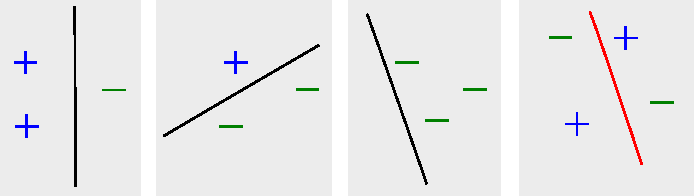
\includegraphics[width=1.0\textwidth]{figs/theory_PRML_shattering.pdf}
								\caption{A linear classifier in $\mathbb{R}^D$ can shatter $D+1$ points.  Here, in the first 3 examples, a line in $\mathbb{R}^2$ is able to shatter 3 points.  However, in the fourth example, it is unable to shatter 4 points.}
								\label{fig:shattering}
								\end{figure}


%================================
\section{Experiments}
%================================
In this section, we experiment with 4 RVQ decode methods:



We start with some trivial scalar examples where the training and test sets are the same.  We then move to the other extreme end of the spectrum using random data in high dimensional spaces with several observations and where the training and test sets have the same distributions but have different data.  After these experiments, we will get to tracking examples and use the likelihood formulation we have developed for RVQ.

\subsection{$S_{trg}=\{1,2,3,4,5,6,7\}$}
%-------------------------------------------------------------

\begin{table}
\centering
\subtable[3x{\color{red}\textbf 2}]{\begin{tabular}{|c|c|}\hline 
2.5  & 6\\
-1  & 1\\
-0.5  & 0.5\\\hline
\end{tabular}}\hspace{0.2in}
\subtable[2x{\color{red}\textbf 3}]{\begin{tabular}{|c|c|c|}\hline
-1 & 6 & 4\\
-1 & 1 & 0\\\hline
\end{tabular}}\hspace{0.2in}
\subtable[2x{\color{red}\textbf 4}]{\begin{tabular}{|c|c|c|c|}\hline
1 & 6.5 & 4 & 2\\
-1 & 1 & -0.5 & 0.5\\\hline
\end{tabular}}\hspace{0.2in}
\subtable[2x{\color{red}\textbf 5}]{\begin{tabular}{|c|c|c|c|c|}\hline
1 & 6.5 & 4.5 & 2 & 3\\
-0.5 & 0.5 & 0 & 0 &0\\\hline
\end{tabular}}\hspace{0.2in}
\subtable[2x{\color{red}\textbf 6}]{\begin{tabular}{|c|c|c|c|c|c|}\hline
1 & 6.5 & 4 & 2 & 3 &5\\
-0.5 & 0.5 & 0 & 0 &0 &0\\\hline
\end{tabular}}\hspace{0.2in}
\subtable[1x{\color{red}\textbf 7}]{\begin{tabular}{|c|c|c|c|c|c|c|}\hline
1 & 7 & 4 & 2 & 3 &5 &6\\\hline
\end{tabular}}
\caption{Designing RVQ codebooks with increasing code-vectors per stage, $m$ = {\color{red}\textbf {2, 3, 4, 5, 6, 7}}.  The training set is $S_{trg}=\{1,2,3,4,5,6,7\}$}
\label{table:1_to_7}
\end{table}

Table~\ref{table:1_to_7} gives an example of designing RVQ codebooks for a trivial  training set in $\mathbb{R}$ that contains only 7 training points, $S_{trg}=\{1,2,3,4,5,6,7\}$.

For $m={\color{red}\textbf 2}$, case, 
For the 3x{\color{red}\textbf 2} case, 

\subsection{Integers, Z=$\{4, 6, 8, 10, 20, 22, 24, 26\}$}
%-------------------------------------------------------------
We train RVQ codebooks with $m=2, 3, \ldots, 16$ on the set of scalars, S=$\{4, 6, 8, 10, 20, 22, 24, 26\}$.  The resulting codebook for the 8x2 case is shown graphically in Figure~\ref{fig:aRVQ_4_6_8_10_20_22_24_26}.  In this initial experiment, the test data is the same as the training data.  Also shown in the figure is the decode path taken by the 4 methods through the RVQ trellis to to decode the number 8.  For monR, when reconstruction reaches 7 in the very first stage, rms error is 1.  However, both next stage codevectors decrease rmse which is why monR exits at this point.  All other methods are able to decode 8 correctly.  These results are shown in Figure~\ref{fig:aRVQ_4_6_8_10_20_22_24_26}.  
  
 
\subsection{Integers, Z=$\{1, 2, \ldots 256\}$}
%------------------------------------------------
In this experiment, we train several RVQ codebooks $m=2, 3, \ldots, 16$ on the set of scalars, S=$\{1, 2, \ldots 256\}$.  The resulting codebook for the 8x2 case is shown graphically in Figure~\ref{fig:aRVQ_1_to_256}.  In this initial experiment, the test data is the same as the training data.  Also shown in the figure is the decode path taken by the 4 methods through the RVQ trellis to to decode the number 13.  For monR, when reconstruction reaches 16.5, rms error is 3.5.  However, both next stage codevectors decrease rmse which is why monR exits at this point.  All other methods are able to decode 13 correctly.   These results are shown in Figure~\ref{fig:aRVQ_1_to_256}. 

\subsection{Gaussian random variables in $\mathbb{R}^{1089}$}
%------------------------------------------------
In this experiment, we train RVQ codebooks with $m=2, 3, \ldots, 16$ on 100 realizations of a unit-variance Gaussian random variable in $\mathbb{R}^{1089}$.  Decoding is then done on a different 100 realizations of a unit-variance Gaussian random variable in $\mathbb{R}^{1089}$.  This experiment is repeated 10 times and the results are averaged and displayed in Figure~\ref{fig:aRVQ_gaussian_rand}.  This experiment is then repeated for a uniform random variable. 

\subsection{Uniform random variables in $\mathbb{R}^{1089}$}
%------------------------------------------------
In this experiment, all details are exactly the same as the Gaussian random variable, except that we've used a uniform random variable.  The results are given in Figure~\ref{fig:aRVQ_uniform_rand}.





\subsection{Images}
%------------------------------------------------
In this experiment, we use actual images from our tracking dataset.  In tracking, a bootstrapping procedure normally involves manually segmenting a target of interest and storing its $x, y, w, h, \theta$ parameters.  These parameters are then converted to an affine 6-tuple.  This 6-tuple allows warping the segmented target onto a user defined rectangular grid.  This warping has the advantage of allowing the target to have a canonical representation with standard size.  Moreover, it will be in upright position.  This can be useful in learning a basis for PCA or generating a codebook for RVQ.  For the purposes of tracking, this initial affine 6-tuple can be used to initialize a particle filter.  The particle filter then generates $N_p$ 6-tuples, and uses the same warping procedure to create $N_p$ canonical targets.  The best one according to a user defined criterion is picked and its affine parameters are then used to generate $N_p$ affine 6-tuples in the next frame and so on.  Notice that in all cases, the target snippets are generated using affine 6-tuples.



In certain cases, we may not have an affine 6-tuple, or manual segmentation may be difficult, but we may need to extract a target of interest.  In cases where running a feature detector is possible, we could extract features of interest from the target of interest.  If we can beforehand determine the position of those features in our canonical grid, then an affine mapping matrix can be computed between the feature points of interest in an image and their positions in the canonical grid.  Note that we would need to determine the positions of those features on our canonical grid only once, and then for every subsequent frame, we could run a feature detector and compute our desired  affine 6-tuple from mapping those features to the features on the canonical grid.

In this experiment, we use the approach of extracting snippets from feature points.  However, in this case, we have ground truth feature points.  Extracted snippets are shown in Figure~\ref{fig:Dudek_1_to_100}.  Training and test rms errors for this experiment are given in Figure~\ref{fig:aRVQ_Dudek_first_100}.  Codebooks are given in Figure~\ref{fig:RVQ_Dudek_codebook}.  Results are shown in Figure~\ref{fig:aRVQ_Dudek_first_100}.




\subsection{Training images with noise, test one image}
%------------------------------------------------
Next, we pick the same snippets as in Figure~\ref{fig:Dudek_1_to_100} but assume that there is noise in the tracker decisions, and at every frame, a slightly incorrect snippet was picked.  In particular, we add gaussian noise with 0 mean and 0.1 standard deviation to the ground truth affine parameters $\theta, \lambda_1, \lambda_2, \phi, t_x, t_y$.  These training snippets are shown in Figure~\ref{fig:aRVQ_dudek_first_100rand_snippets}.  The results shown in Figure~\ref{fig:aRVQ_Dudek_first_100_rand} again show that nulE produces least reconstruction rms error.

\subsection{Training images with noise, test several images}
%------------------------------------------------
This experiment is exactly the same as the previous one except that we test several snippets, some of which also have occlusions.

%================================
\section{Results}
%================================







We carried out experiments on two opposite ends of the spectrum. 

On the simplest side were deterministic data experiments where the training and test sets were the same.  maxP and RofE naturally did well.  monR nevertheless was unable to decode correctly in quite a few occasions and the reasons have been examined in earlier sections.  

On the extremely difficult side of things were the random data experiments with high dimensional data with several observations.  In these experiments, nulE performed the best.  The reason is that even if a subsequent stage does not decrease rms error, nulE can rely on subsequent lower energy stages to nudge down its rms error.  

%For the Gaussian random variable experiments, training data rms error decreased with increasing code-vectors per stage.  However, test error for maxQ and RofE increased while test error for nulE and monR did not show a clear trend.  For uniform random variable experiments, both training and test rms errors increased with number of code-vectors per stage.  It appears that whereas the uniform distribution has a clear trend, increasing error with code-vectors per stage, finding a clear trend with the gaussian random variable is more challenging.

It may be noted that the rms errors obtained were quite high for the random data sets, compared to the actual values of the signal.  The reason is quite clearly that the datasets we picked were extremely challenging.  We have seen much better performance with data sets in which correlations in the data can be exploited, for instance in images.

%================================
\section{Conclusions}
%================================
Over the spectrum of low and high dimensional deterministic or random data, nulE performs the best.





\clearpage
\newpage
\subsection{Integers, Z=$\{4, 6, 8, 10, 20, 22, 24, 26\}$}
%-------------------------------------------------------------
								\begin{figure}[h!]
								\centering
								\subfigure[3x2 RVQ codebook.  The reconstruction path taken through the codebook by the integer 8 is shaded dark.  Notice that monR is the only method unable to correctly decode the integer 8 and produces a 7 instead.  monR also incorrectly decodes 6, 8, 23 and 24.]{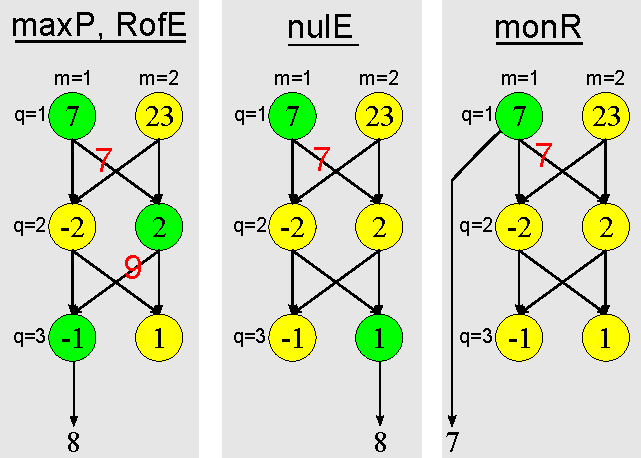
\includegraphics[width=0.5\textwidth]{figs/RVQ_CAC_toyExample_3x2.pdf}}
						\subfigure[3x2 TSVQ codebook and reconstruction path taken by the number 8.]{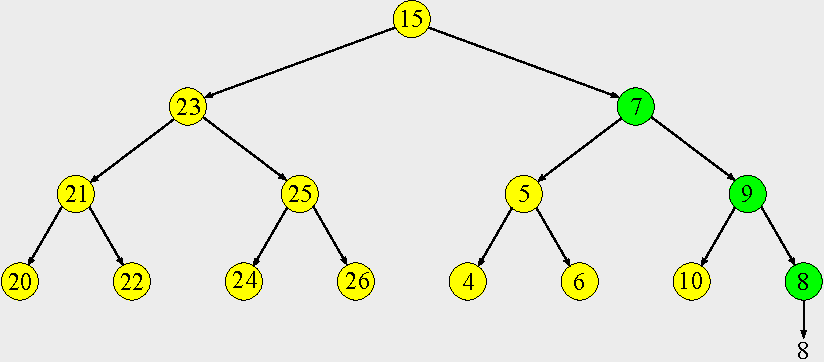
\includegraphics[width=0.85\textwidth]{figs/TSVQ_toyExample_3x2.pdf}}
								\caption{RVQ and TSVQ codebooks generated using the training data $S_{trg}~=~\{4, 6, 8, 10, 20, 22, 24, 26\}$.}
								\end{figure}
															


								\begin{table}[h]
								\centering
								\begin{tabular}{|l|c|c|c|c|c|}
\hline
&\textbf{Trng}&\textbf{maxQ}&\textbf{RofE}&\textbf{nulE}&\textbf{monR}\\\hline
\textbf{3x2}&0.0000&0.0000&0.0000&0.0000&0.7071\\\hline
\textbf{3x3}&0.0001&0.0001&0.0001&0.0001&0.0001\\\hline
\textbf{2x4}&0.0000&0.0000&0.0000&0.0000&0.0000\\\hline
\textbf{2x5}&0.0000&0.0000&0.0000&0.0000&0.0000\\\hline
\textbf{2x6}&0.0000&0.0000&0.0000&0.0000&0.0000\\\hline
\textbf{2x7}&0.0000&0.0000&0.0000&0.0000&0.0000\\\hline
\textbf{1x8}&0.0000&0.0000&0.0000&0.0000&0.0000\\\hline
\textbf{mean}&0.0000&0.0000&0.0000&0.0000&0.101\\\hline
\end{tabular}

								\caption{RVQ reconstruction rms errors.  The training set is $S_{\textrm{trg}}=S_{\textrm{tst}}=\{4, 6, 8, 10, 20, 22, 24, 26\}$.  As the number of templates per stage $m$ is increased, less and less stages are needed for perfect reconstruction.}
								\label{fig:aRVQ_4_6_8_10_20_22_24_26}
								\end{table}
\clearpage
\newpage
\subsection{Integers, Z=$\{1, 2, \ldots 256\}$}
%------------------------------------------------
								\begin{figure}[h]
								\centering
								\subfigure[8x2 RVQ codebook.  The reconstruction path taken through the codebook by the integer 13 is shaded dark.  Notice that monR is the only method unable to correctly decode the integer 13 and produces 16.5 instead.]{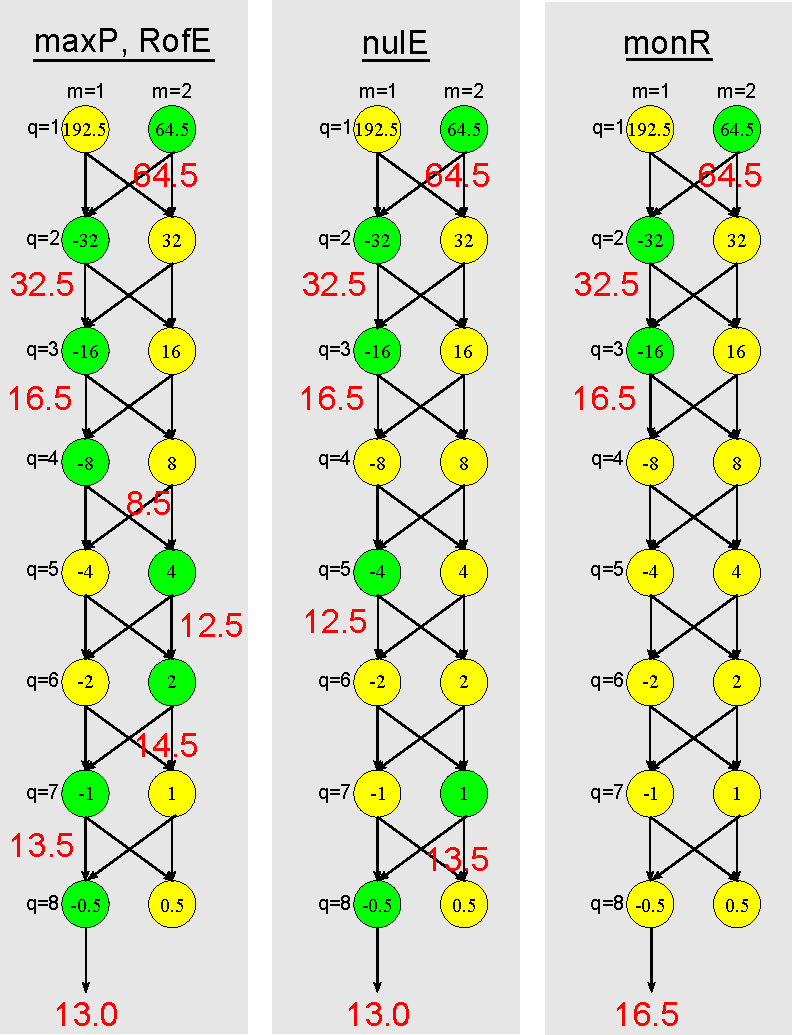
\includegraphics[height=3in]{figs/RVQ_CAC_toyExample_8x2.pdf}}\hspace{0.1in}
								\subfigure[For the 8x2 RVQ codebook, input and decoded outputs produced by monR.  Notice quite a few incorrect reconstructions.  In contrast, maxP, RofE and nulE all produce perfect reconstructions.]{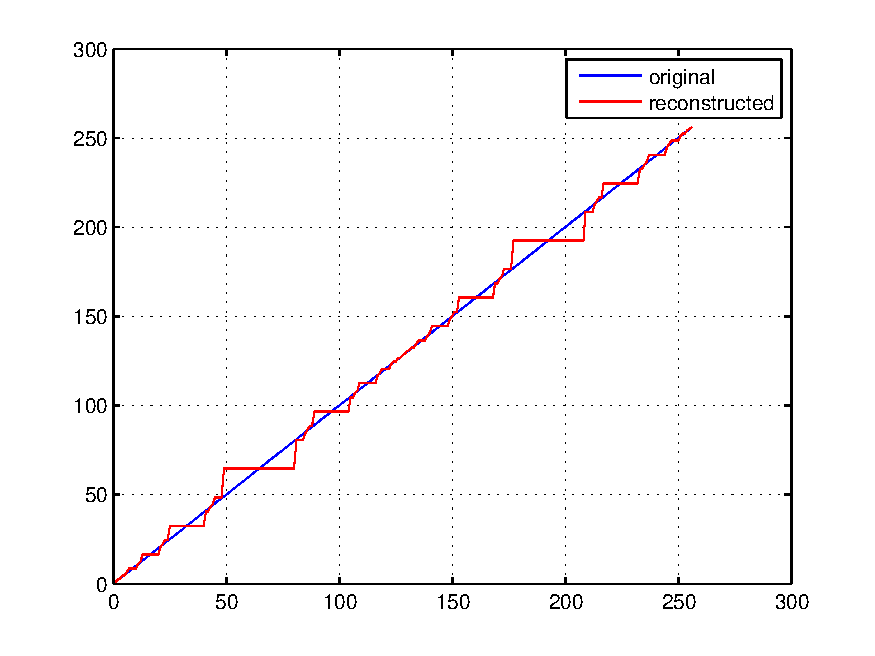
\includegraphics[height=2in]{figs/RVQ_CAC_toyExample_8x2_monR.pdf}}
								\subtable{\begin{tabular}{|l|c|c|c|c|c|}
\hline
&\textbf{Trng}&\textbf{maxQ}&\textbf{RofE}&\textbf{nulE}&\textbf{monR}\\\hline
\textbf{8x2}&0.0000&0.0000&0.0000&0.0000&5.2723\\\hline
\textbf{8x3}&0.0000&0.0000&0.0000&0.0015&3.5426\\\hline
\textbf{5x4}&0.0000&0.0000&0.0000&0.0726&0.8745\\\hline
\textbf{5x5}&0.0000&0.0000&0.0000&0.0562&1.0328\\\hline
\textbf{4x6}&0.0625&0.0625&0.0625&0.1024&0.6740\\\hline
\textbf{4x7}&0.0000&0.0000&0.0000&0.0284&0.3084\\\hline
\textbf{4x8}&0.0000&0.0000&0.0000&0.0090&0.2700\\\hline
\textbf{3x9}&0.0000&0.0000&0.0000&0.0043&0.2289\\\hline
\textbf{5x10}&0.0000&0.0000&0.0000&0.0020&0.0889\\\hline
\textbf{3x11}&0.0000&0.0000&0.0000&0.0085&0.1507\\\hline
\textbf{3x12}&0.0000&0.0000&0.0000&0.0255&0.1494\\\hline
\textbf{3x13}&0.0000&0.0000&0.0000&0.0119&0.0827\\\hline
\textbf{3x14}&0.0186&0.0186&0.0186&0.0000&0.0000\\\hline
\textbf{3x15}&0.0153&0.0153&0.0153&0.0007&0.0068\\\hline
\textbf{3x16}&0.0011&0.0011&0.0011&0.0006&0.0043\\\hline
\textbf{mean}&0.0065&0.0065&0.0065&0.0216&0.8458\\\hline
\end{tabular}
}
								\subfigure{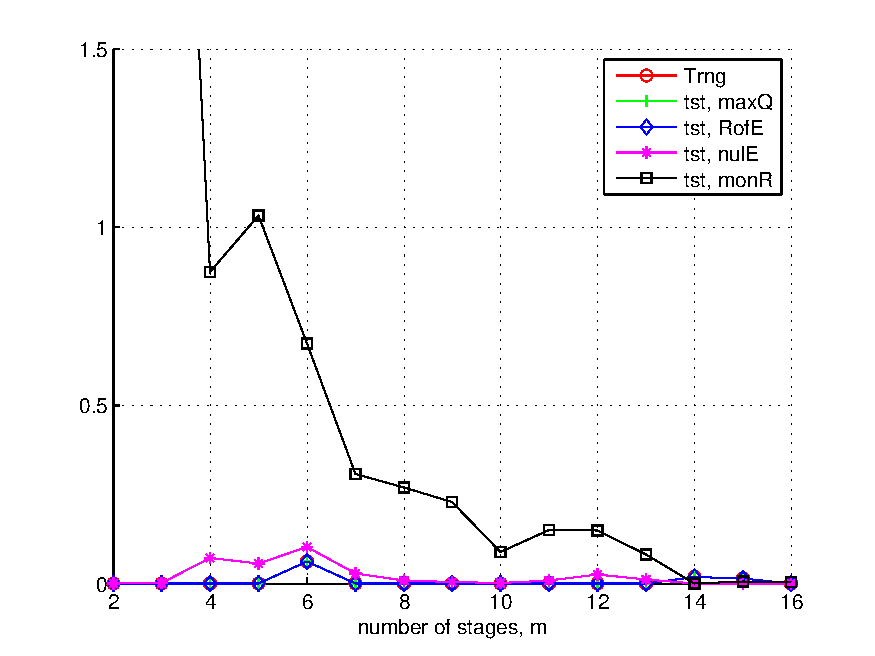
\includegraphics[width=0.5\textwidth]{figs/aRVQ_1_to_256.pdf}}
								\caption{Training set  $S_{\textrm{trg}}=\{1, 2, \ldots 256\}$, , the test set $S_{\textrm{tst}}$ is the same as the training set.}
								\label{fig:aRVQ_1_to_256}
								\end{figure}

\clearpage
\newpage
\subsection{Gaussian random variables in $\mathbb{R}^{1089}$}
%------------------------------------------------

								\begin{figure}[h]
								\centering
								\subtable{\begin{tiny}\begin{tabular}{|l|c|c|c|c|c|}
\hline
&\textbf{Trng}&\textbf{maxQ}&\textbf{RofE}&\textbf{nulE}&\textbf{monR}\\\hline
\textbf{m=2}&1.0434&1.0789&1.0789&1.0735&1.0748\\\hline
\textbf{m=3}&1.0188&1.0770&1.0770&1.0691&1.0708\\\hline
\textbf{m=4}&0.9861&1.0807&1.0807&1.0695&1.0709\\\hline
\textbf{m=5}&0.9656&1.0896&1.0892&1.0721&1.0731\\\hline
\textbf{m=6}&0.9433&1.0904&1.0904&1.0725&1.0733\\\hline
\textbf{m=7}&0.9092&1.0987&1.0987&1.0690&1.0692\\\hline
\textbf{m=8}&0.8890&1.1064&1.1064&1.0720&1.0724\\\hline
\textbf{m=9}&0.8739&1.1099&1.1096&1.0687&1.0691\\\hline
\textbf{m=10}&0.8468&1.1288&1.1286&1.0750&1.0752\\\hline
\textbf{m=11}&0.8314&1.1471&1.1468&1.0739&1.0740\\\hline
\textbf{m=12}&0.9110&1.1471&1.1471&1.0731&1.0735\\\hline
\textbf{m=13}&1.0792&1.2407&1.2404&1.0705&1.0705\\\hline
\textbf{m=14}&0.9386&1.1561&1.1558&1.0692&1.0692\\\hline
\textbf{m=15}&0.7999&1.1546&1.1537&1.0772&1.0774\\\hline
\textbf{m=16}&0.9250&1.1633&1.1605&1.0722&1.0722\\\hline
\textbf{mean}&0.9308&1.1246&1.1242&1.0718&1.0724\\\hline
\end{tabular}
\end{tiny}}
								\subfigure{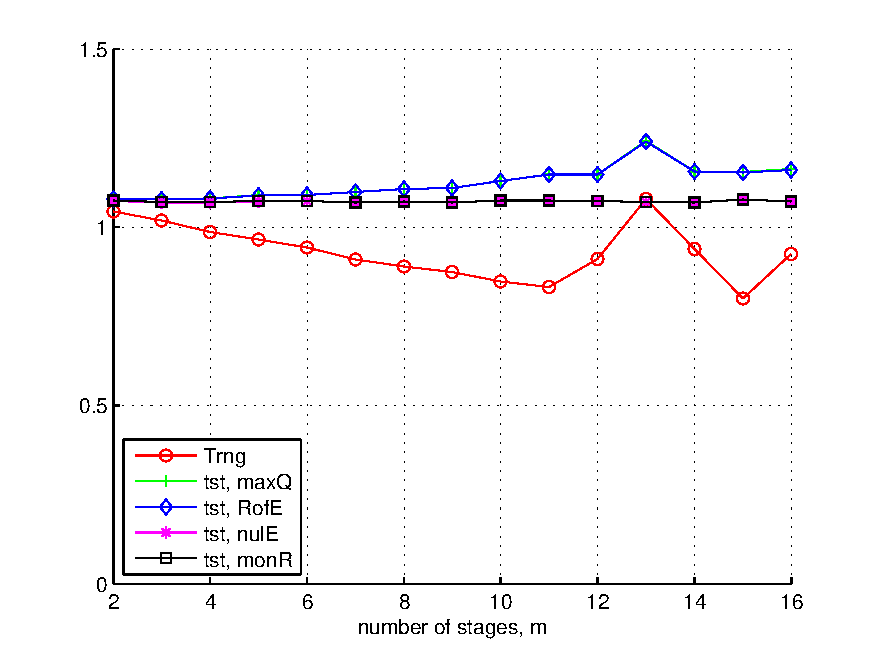
\includegraphics[width=0.6\textwidth]{figs/aRVQ_gaussian_rand.pdf}}
								\caption{Reconstruction rms errors for different values of RVQ code-vectors per stage, $m$.  The training set $S_{\textrm{trg}}$ consists of 100 realizations of a zero-mean unit-variance Gaussian random variable, $S_{\textrm{trg}} \sim \mathcal{N}(0, 1) \in \mathbb{R}^{1089}$.  The test set $S_{\textrm{tst}}$ consists of 100 different realizations of a zero-mean unit-variance Gaussian random variable 	 $S_{\textrm{tst}} \sim \mathcal{N}(0, 1) \in \mathbb{R}^{1089}$, $S_{\textrm{tst}} \neq S_{\textrm{trg}}$.  Notice that the error is close to the variance of the random variable. }
								\label{fig:aRVQ_gaussian_rand}
								\end{figure}

\clearpage
\newpage
\subsection{Uniform random variables in $\mathbb{R}^{1089}$}
%------------------------------------------------
								\begin{figure}[h]
								\centering
								\subtable{\begin{tiny}\begin{tabular}{|l|c|c|c|c|c|}
\hline
&\textbf{Trng}&\textbf{maxQ}&\textbf{RofE}&\textbf{nulE}&\textbf{monR}\\\hline
\textbf{m=2}&0.2900&0.3167&0.3167&0.2959&0.2959\\\hline
\textbf{m=3}&0.2897&0.3395&0.3395&0.3007&0.3008\\\hline
\textbf{m=4}&0.2929&0.3469&0.3468&0.3039&0.3039\\\hline
\textbf{m=5}&0.3028&0.3578&0.3578&0.3057&0.3057\\\hline
\textbf{m=6}&0.2994&0.3831&0.3829&0.3160&0.3160\\\hline
\textbf{m=7}&0.3083&0.3928&0.3926&0.3193&0.3193\\\hline
\textbf{m=8}&0.3283&0.4149&0.4149&0.3243&0.3243\\\hline
\textbf{m=9}&0.3518&0.4132&0.4132&0.3286&0.3286\\\hline
\textbf{m=10}&0.3766&0.4444&0.4425&0.3366&0.3366\\\hline
\textbf{m=11}&0.4197&0.4786&0.4786&0.3392&0.3395\\\hline
\textbf{m=12}&0.4288&0.4626&0.4626&0.3367&0.3367\\\hline
\textbf{m=13}&0.6027&0.6428&0.6428&0.3727&0.3727\\\hline
\textbf{m=14}&0.4492&0.4749&0.4749&0.4011&0.4019\\\hline
\textbf{m=15}&0.4243&0.4773&0.4765&0.3866&0.3869\\\hline
\textbf{m=16}&0.5307&0.5676&0.5676&0.4028&0.4053\\\hline
\textbf{mean}&0.3797&0.4342&0.4340&0.3380&0.3383\\\hline
\end{tabular}
\end{tiny}}
								\subfigure{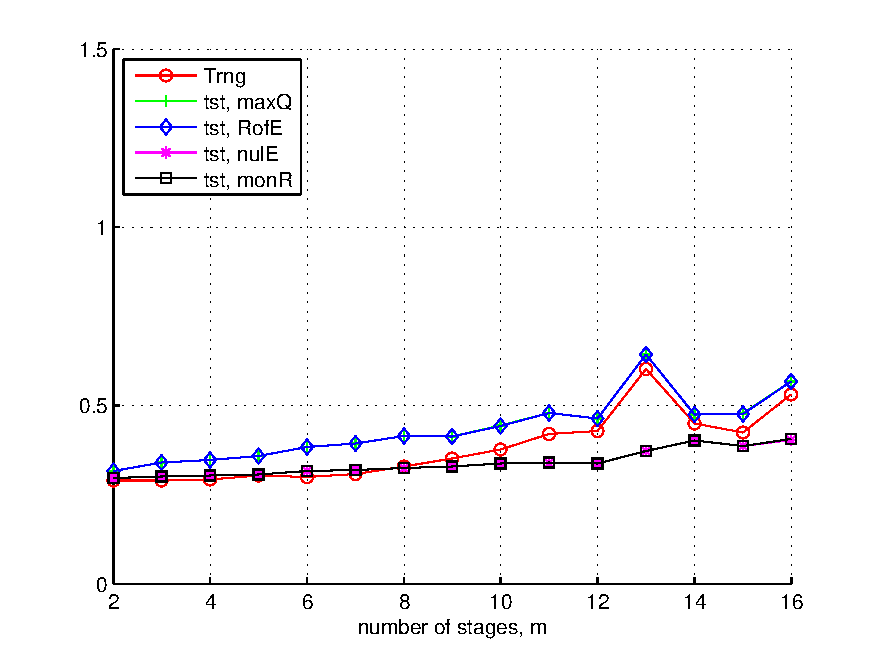
\includegraphics[width=0.6\textwidth]{figs/aRVQ_uniform_rand.pdf}}
								\caption{Reconstruction rms errors for different values of RVQ code-vectors per stage, $m$.  The training set $S_{\textrm{trg}}$ consists of 100 realizations of a uniform random variable, $S_{\textrm{trg}} \sim U[0, 1] \in \mathbb{R}^{1089}$.  The test set $S_{\textrm{tst}}$ consists of 100 different realizations of a zero-mean uniform random variable 	 $S_{\textrm{tst}} \sim U[0, 1] \in \mathbb{R}^{1089}$, $S_{\textrm{tst}} \neq S_{\textrm{trg}}$.}
								\label{fig:aRVQ_uniform_rand}
								\end{figure}

\clearpage
\newpage
\subsection{Images}
%------------------------------------------------
								\begin{figure}[h]
								\centering
								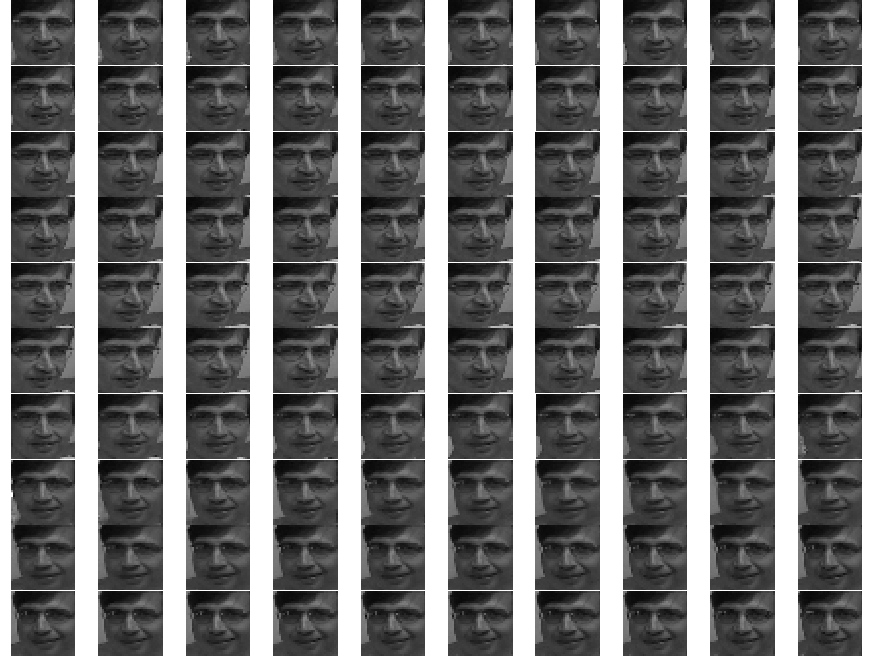
\includegraphics[width=0.55\textwidth]{figs/Dudek_snippets_frames_1_to_100.pdf}
								\caption{Training snippets extracted using ground truth information, first 100 frames of Dudek sequence.}
								\label{fig:Dudek_1_to_100}
								\end{figure}	

								\begin{figure}[h]
								\centering
								\subfigure[8x2.]{\fbox{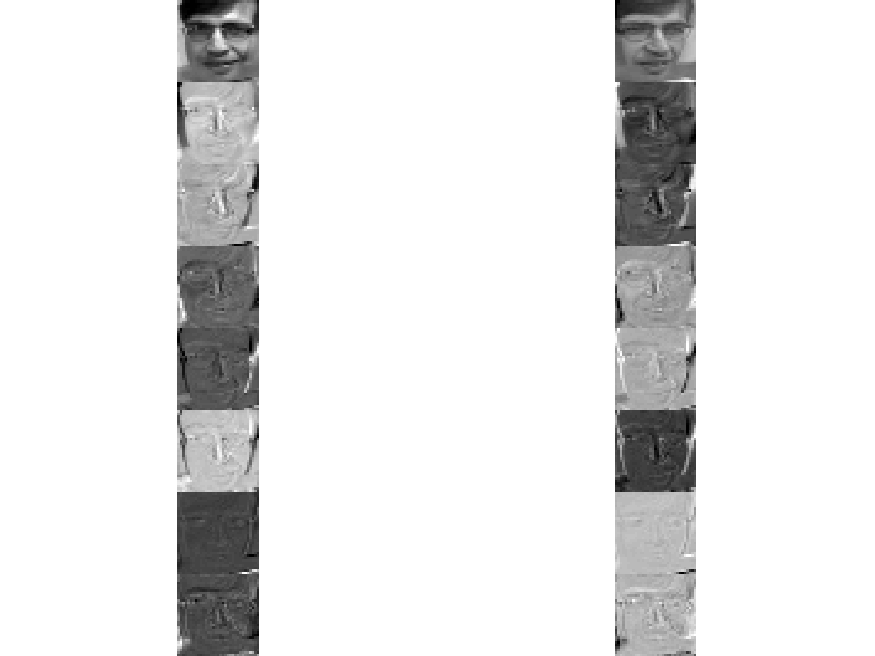
\includegraphics[height=1.5in]{figs/Dudek_snippets_frames_1_to_100_8x2_RVQ.pdf}}}
								\subfigure[8x4.]{\fbox{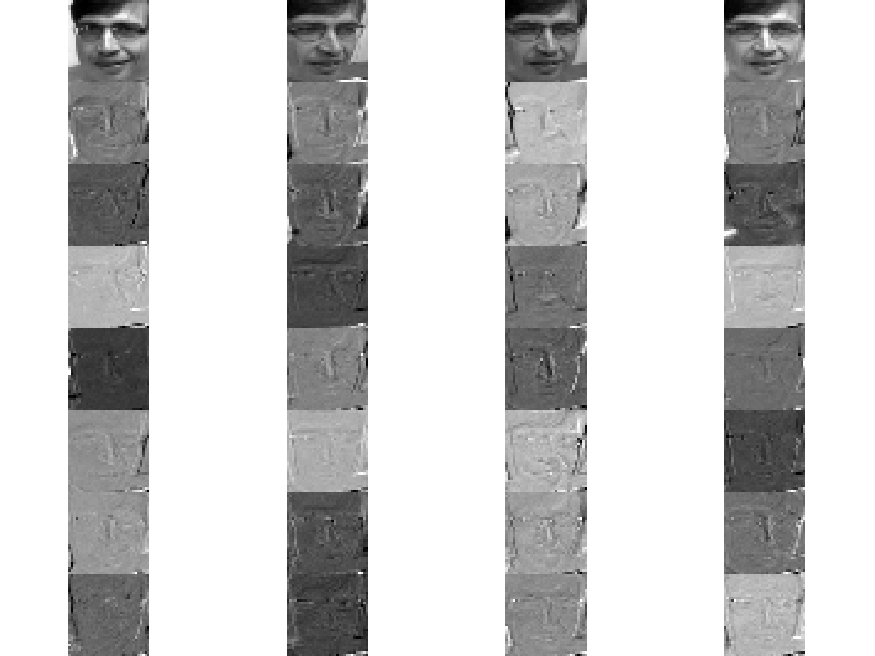
\includegraphics[height=1.5in]{figs/Dudek_snippets_frames_1_to_100_8x4_RVQ.pdf}}}
								\subfigure[8x8.]{\fbox{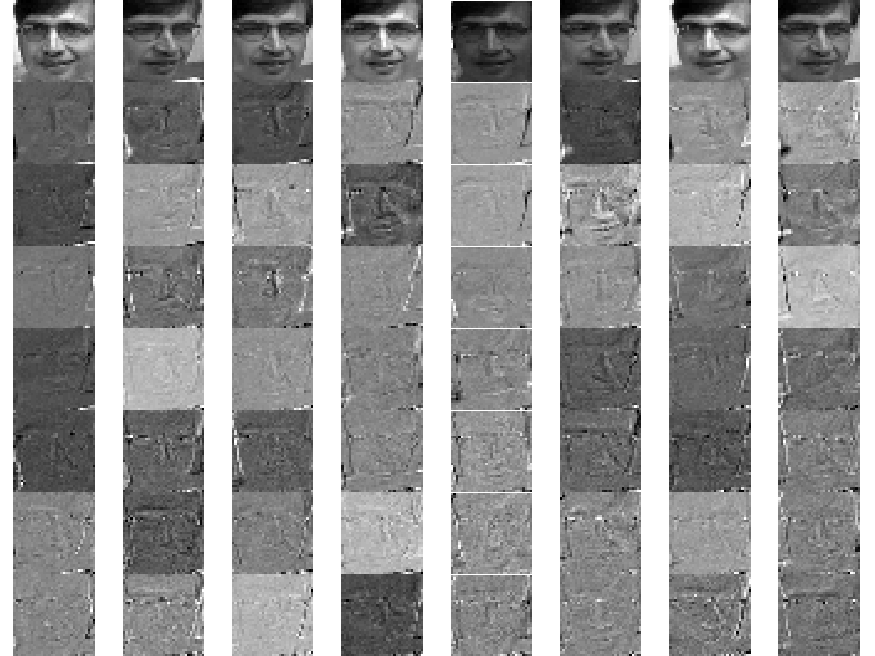
\includegraphics[height=1.5in]{figs/Dudek_snippets_frames_1_to_100_8x8_RVQ.pdf}}}
								\subfigure[8x16.]{\fbox{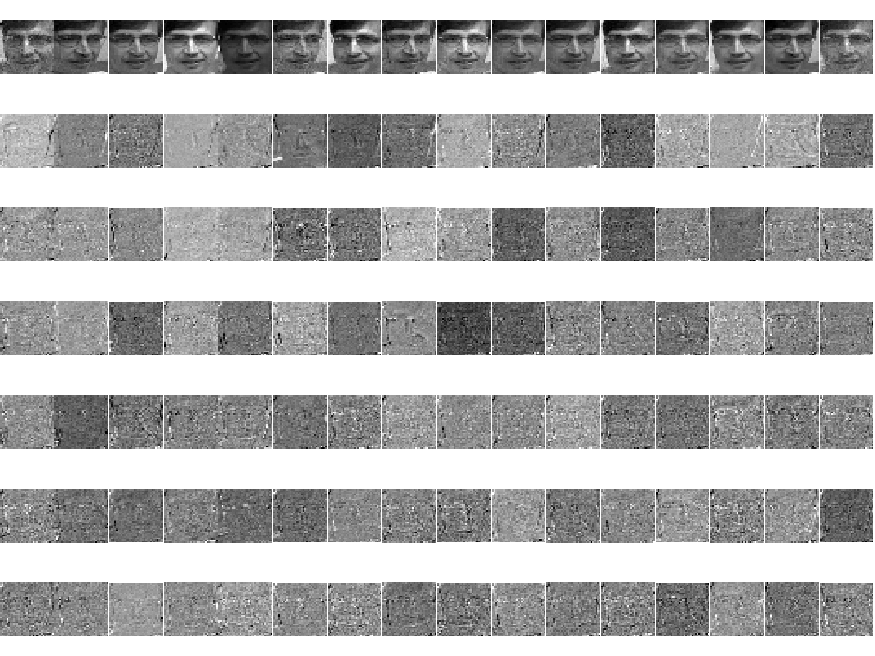
\includegraphics[height=2.5in]{figs/Dudek_snippets_frames_1_to_100_8x16_RVQ.pdf}}}
								\caption{RVQ codebooks for the snippets in Figure~\ref{fig:Dudek_1_to_100}.  Intensities have been scaled to be able to view lower energy code-vectors.}
								\label{fig:RVQ_Dudek_codebook}
								\end{figure}


								\begin{figure}
								\centering
								\subtable{\begin{tiny}\input{tables/aRVQ_Dudek_first_100.tex}\end{tiny}}
								\subfigure{\includegraphics[width=0.6\textwidth]{figs/aRVQ_Dudek_first_100.pdf}}
								\caption{Reconstruction rms errors for different values of RVQ code-vectors per stage, $m$ for the first 100 target snippets in the Dudek sequence.  These snippets can be seen in Figure~\ref{fig:Dudek_1_to_100}.}
								\label{fig:aRVQ_Dudek_first_100}
								\end{figure}

\clearpage
\newpage
\subsection{Training images with noise, test one image}
%------------------------------------------------


								\begin{figure}[h]
								\centering
								\subfigure[Training snippets.]{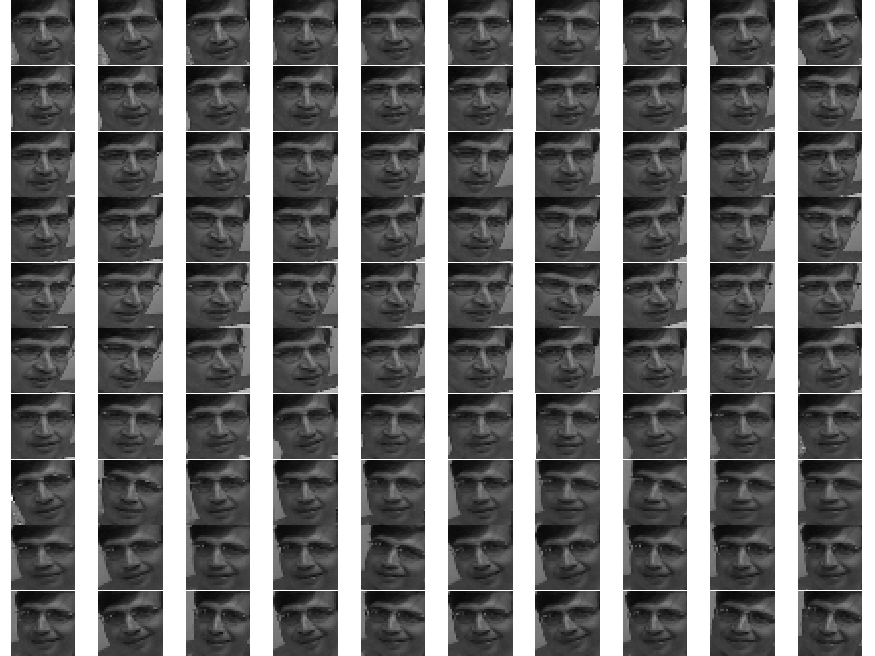
\includegraphics[width=0.55\textwidth]{figs/aRVQ_dudek_first_100rand_snippets.pdf}}
								\subfigure[Test snippet.]{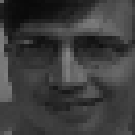
\includegraphics[width=0.15\textwidth]{figs/dataset_Dudek_snippet_00101.png}}
								\caption{The training snippets were extracted using ground truth information from the first 100 frames of the Dudek sequence.  The affine parameters of the ground truth affine parameters $\theta, \lambda_1, \lambda_2, \phi, t_x, t_y$ were perturbed with a zero-mean gaussian random variable with 0.1 standard deviation.  This was done to simulate a condition in which the tracker does not make perfect decisions on every frame.  Compare with Figure~\ref{fig:Dudek_1_to_100} in which perfect snippets are shown.}
								\label{fig:aRVQ_dudek_first_100rand_snippets}
								\end{figure}

								\begin{figure}
								\centering
								\subtable{\begin{tiny}\begin{tabular}{|l|c|c|c|c|c|}
\hline
&\textbf{Trng}&\textbf{maxQ}&\textbf{RofE}&\textbf{nulE}&\textbf{monR}\\\hline
\textbf{m=2}&9.5600&11.5445&11.5445&10.6894&11.5407\\\hline
\textbf{m=3}&8.0438&10.3221&10.3221&10.3221&10.3221\\\hline
\textbf{m=4}&7.2279&9.8930&9.8930&10.1110&13.5156\\\hline
\textbf{m=5}&6.3219&8.6734&10.6990&8.5766&10.6162\\\hline
\textbf{m=6}&6.0218&9.0967&9.1437&8.9042&9.5178\\\hline
\textbf{m=7}&5.6085&8.3236&8.3236&7.8873&10.8008\\\hline
\textbf{m=8}&4.9347&7.7742&7.7742&7.6583&7.6583\\\hline
\textbf{m=9}&3.7935&8.8903&8.8903&8.5680&11.1848\\\hline
\textbf{m=10}&3.8130&10.2114&10.2856&9.6627&10.2856\\\hline
\textbf{m=11}&4.3059&8.5473&8.5473&8.8143&10.1338\\\hline
\textbf{m=12}&4.9797&10.9766&10.9766&10.8308&10.9307\\\hline
\textbf{m=13}&9.9797&11.5537&11.5537&11.7415&13.5554\\\hline
\textbf{m=14}&7.5239&8.2772&8.2772&10.8795&11.0513\\\hline
\textbf{m=15}&6.3353&10.1674&10.1674&10.6053&10.8589\\\hline
\textbf{m=16}&8.7544&11.3914&12.5073&11.3163&12.5073\\\hline
\textbf{mean}&6.4803&9.7095&9.9270&9.7712&10.9653\\\hline
\end{tabular}
\end{tiny}}
								\subfigure{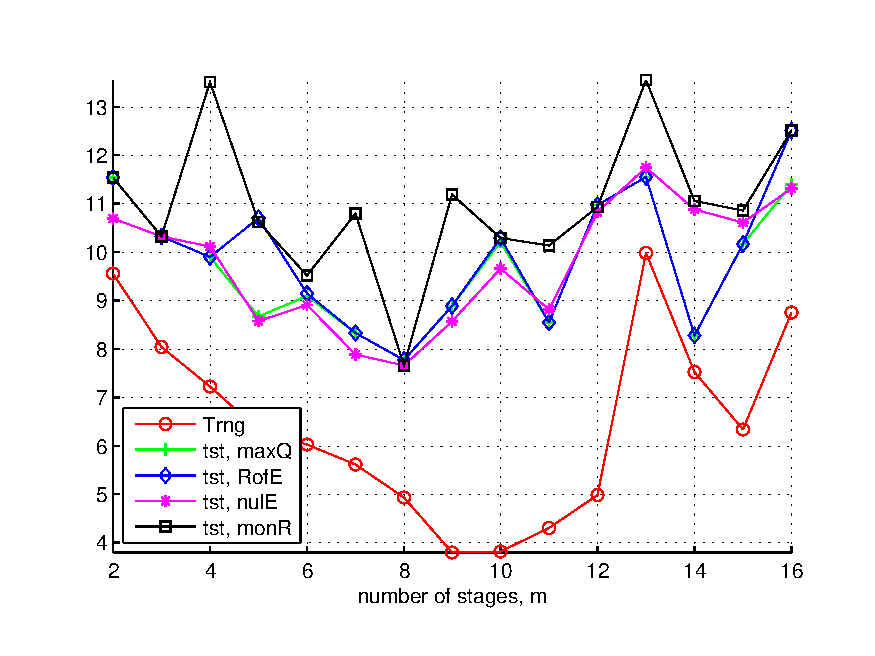
\includegraphics[width=0.6\textwidth]{figs/aRVQ_dudek_first_100rand_101test.pdf}}
								\caption{Reconstruction rms errors for different values of RVQ code-vectors per stage, $m$ with first 100 target snippets in the Dudek sequence randomized with zero-mean gaussian noise with 0.1 standard deviation.  The training snippets can be seen in Figure~\ref{fig:aRVQ_dudek_first_100rand_snippets}.}
								\label{fig:aRVQ_Dudek_first_100_rand}
								\end{figure}



\clearpage
\newpage
\subsection{Training images with noise, test several images}
%------------------------------------------------
Training snippets are similar to the ones in Figure~\ref{fig:aRVQ_dudek_first_100rand_snippets} since exactly the same noise parameters were used.


								\begin{figure}[h!]
								\centering
								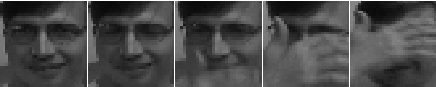
\includegraphics[width=0.55\textwidth]{figs/aRVQ_dudek_first_100_to_105_snippets.pdf}
								\caption{Test snippts.}
								\label{fig:aRVQ_Dudek_first_100_rand}
								\end{figure}


								\begin{figure}[h]
								\centering
								\subtable{\begin{tiny}\begin{tabular}{|l|c|c|c|c|c|}
\hline
&\textbf{Trng}&\textbf{maxQ}&\textbf{RofE}&\textbf{nulE}&\textbf{monR}\\\hline
\textbf{m=2}&9.9127&21.7184&21.7184&21.0123&21.2962\\\hline
\textbf{m=3}&8.4270&21.6515&21.6515&21.2279&22.0090\\\hline
\textbf{m=4}&7.3240&20.9485&21.3400&20.9388&21.3264\\\hline
\textbf{m=5}&6.3207&21.0449&21.2891&21.2035&21.6648\\\hline
\textbf{m=6}&5.8610&21.4626&21.4626&21.4982&21.9101\\\hline
\textbf{m=7}&5.3670&21.4030&21.4686&21.2181&21.5418\\\hline
\textbf{m=8}&4.6272&21.0783&21.8278&20.9523&21.1244\\\hline
\textbf{m=9}&4.3388&21.5432&21.6363&21.3424&21.9305\\\hline
\textbf{m=10}&4.5128&21.1419&21.4674&21.0489&21.6408\\\hline
\textbf{m=11}&4.5271&21.8987&21.8987&21.5153&22.0900\\\hline
\textbf{m=12}&5.1375&21.6045&21.6510&21.3662&21.9312\\\hline
\textbf{m=13}&8.0651&23.0838&23.0838&22.5296&22.8022\\\hline
\textbf{m=14}&10.2941&22.5911&22.6383&22.0515&22.5901\\\hline
\textbf{m=15}&3.6904&21.5804&21.6297&21.4690&21.8980\\\hline
\textbf{m=16}&7.3600&21.9300&21.9094&21.7711&22.0840\\\hline
\textbf{mean}&6.3844&21.6454&21.7782&21.4097&21.8560\\\hline
\end{tabular}
\end{tiny}}
								\subfigure{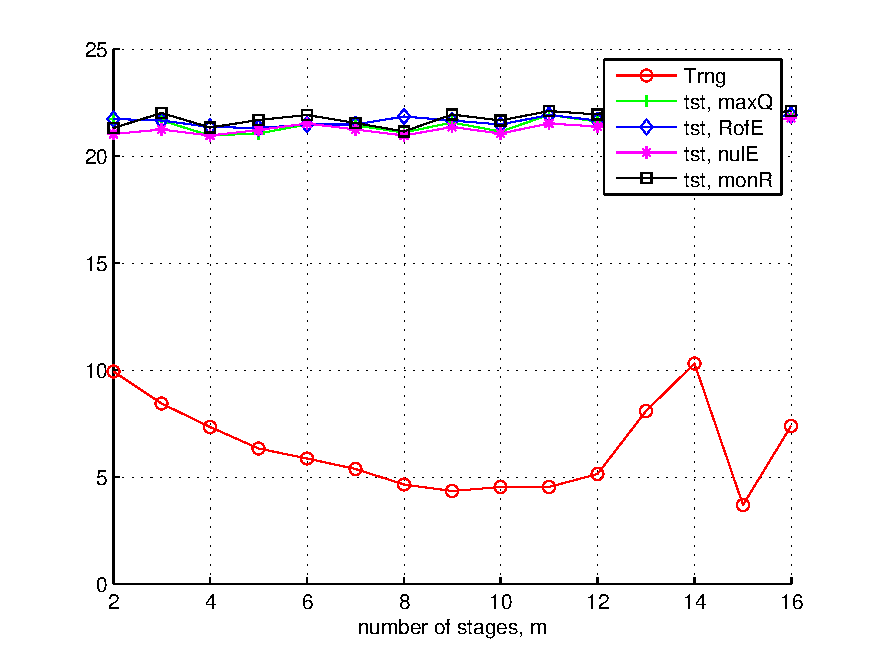
\includegraphics[width=0.6\textwidth]{figs/aRVQ_dudek_first_100rand_5test.pdf}}
								\caption{Reconstruction rms errors for different values of RVQ code-vectors per stage, $m$ with first 100 target snippets in the Dudek sequence randomized with zero-mean gaussian noise with 0.1 standard deviation.  The training snippets can be seen in Figure~\ref{fig:aRVQ_dudek_first_100rand_snippets}.}
								\label{fig:aRVQ_Dudek_first_100_rand}
								\end{figure}




\clearpage
\newpage
\normalsize
\bibliographystyle{ieee}
\bibliography{MyCitations}
\end{document}